%% This is a shared SUNDIALS TEX file with a description of the
%% banded sunmatrix implementation
%%

The banded implementation of the {\sunmatrix} module provided with
{\sundials}, {\sunmatband}, defines the {\em content} field
of \id{SUNMatrix} to be the following structure:
%%
\begin{verbatim} 
struct _SUNMatrixContent_Band {
  sunindextype M;
  sunindextype N;
  sunindextype mu;
  sunindextype ml;
  sunindextype s_mu;
  sunindextype ldim;
  realtype *data;
  sunindextype ldata;
  realtype **cols;
};
\end{verbatim}
%%
A diagram of the underlying data representation in a banded matrix is
shown in Figure \ref{f:sunbandmat}.  A more complete description of the
parts of this \emph{content} field is given below:
\begin{description}
  \item[M] - number of rows
  \item[N] - number of columns (\id{N} = \id{M})
  \item[mu] - upper half-bandwidth, $0 \le$ \id{mu} $<$ \id{N}
  \item[ml] - lower half-bandwidth, $0 \le$ \id{ml} $<$ \id{N}
  \item[s\_mu] - storage upper bandwidth, \id{mu} $\le$ \id{s\_mu} $<$ \id{N}.
    The LU decomposition routines in the associated {\sunlinsolband}
    and {\sunlinsollapband} modules write the LU factors into the
    storage for A. The upper triangular factor U, however, may have  
    an upper bandwidth as big as min(\id{N}-1,\id{mu}+\id{ml}) because of 
    partial pivoting. The \id{s\_mu} field holds the upper
  half-bandwidth allocated for A.
  \item[ldim] - leading dimension (\id{ldim} $\ge$ \id{s\_mu}+\id{ml}+1)
  \item[data] - pointer to a contiguous block of \id{realtype} variables.
    The elements of the banded matrix are stored columnwise
    (i.e.~columns are stored one on top of the other in memory). Only
    elements within the specified half-bandwidths are stored.     
    \id{data} is a pointer to \id{ldata} contiguous locations   
    which hold the elements within the band of A.  
  \item[ldata] - length of the data array
    ($=$ \id{ldim}$\cdot N$) 
  \item[cols] - array of pointers. \id{cols[j]} is a pointer to the
    uppermost element within the band in the j-th column. This pointer
    may be treated as an array indexed from \id{s\_mu}$-$\id{mu} (to
    access the uppermost element within the band in the j-th column)
    to \id{s\_mu}$+$\id{ml} (to access the lowest element within the
    band in the j-th column). Indices from $0$ to
    \id{s\_mu}$-$\id{mu}$-1$ give access to extra storage elements
    required by the LU decomposition function.
    Finally, \id{cols[j][i-j+s\_mu]} is the $(i,j)$-th element with
    $j-$\id{mu} $\le i \le j+$\id{ml}.  
\end{description}
%%
%%--------------------------------------------
%%
\begin{figure}
\centerline{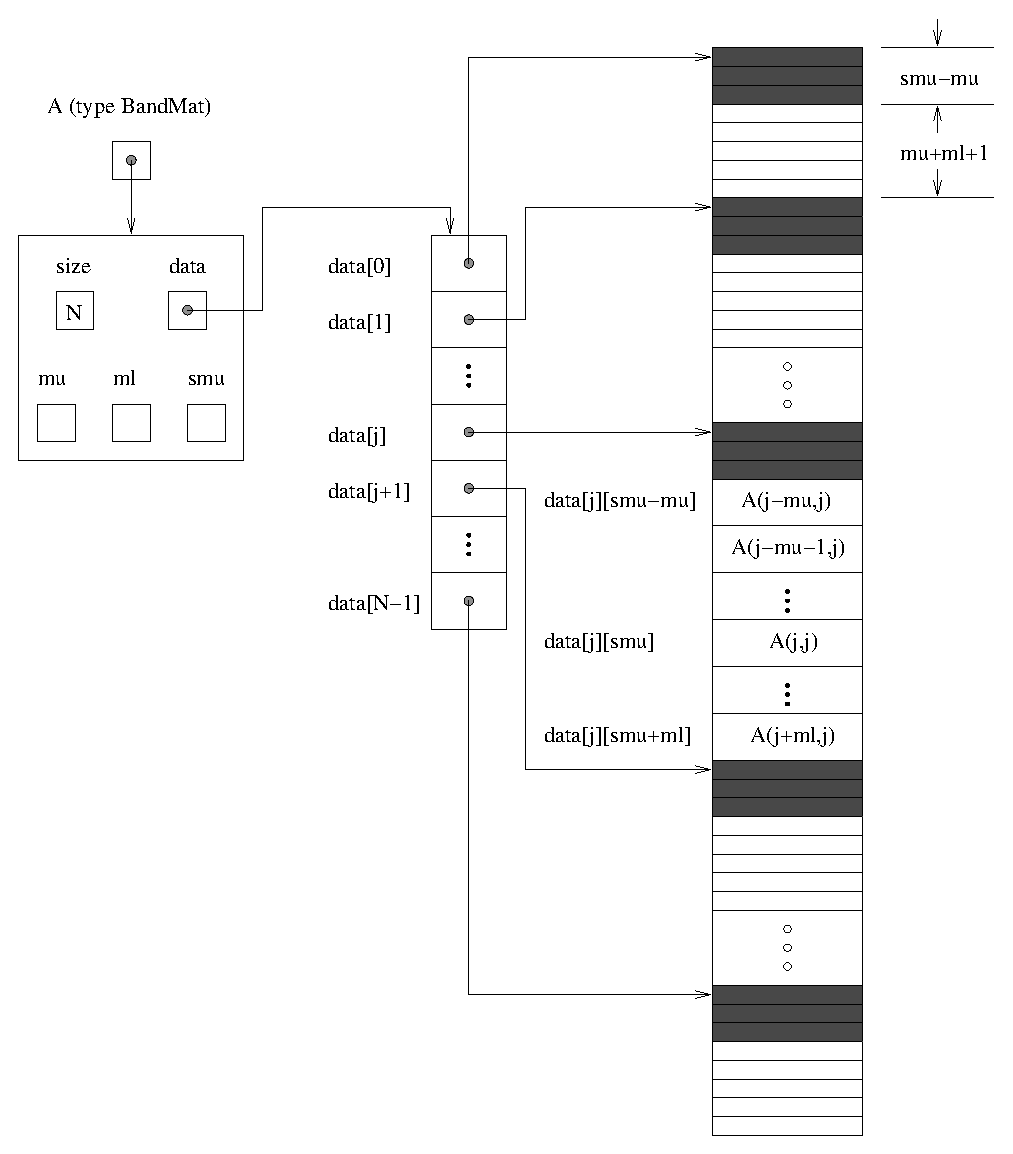
\includegraphics[width=4.5 in]{bandmat}}
\caption[Diagram of the storage for a {\sunmatband} object]
  {Diagram of the storage for the {\sunmatband} module. Here \id{A} is an
  $\id{N} \times \id{N}$ band matrix with upper and lower half-bandwidths \id{mu}
  and \id{ml}, respectively. The rows and columns of \id{A} are
  numbered from $0$ to $\id{N}-1$ and the ($i,j$)-th element of \id{A} is
  denoted \id{A(i,j)}. The greyed out areas of the underlying
  component storage are used by the associated {\sunlinsolband}
  linear solver.}\label{f:sunbandmat}
\end{figure}

\noindent The header file to include when using this module 
is \id{sunmatrix/sunmatrix\_band.h}. The {\sunmatband} module
is accessible from all {\sundials} solvers \textit{without}
linking to the \\
\id{libsundials\_sunmatrixband} module library. \\

\noindent The following macros are provided to access the
content of a {\sunmatband} matrix. The prefix \id{SM\_} in the names
denotes that these macros are for \emph{SUNMatrix} implementations,
and the suffix \id{\_B} denotes that these are specific to
the \emph{banded} version.
%%
\begin{itemize}

\item \ID{SM\_CONTENT\_B}
    
  This routine gives access to the contents of the
  banded \id{SUNMatrix}.
  
  The assignment \id{A\_cont} $=$ \id{SM\_CONTENT\_B(A)} sets           
  \id{A\_cont} to be a pointer to the banded \id{SUNMatrix} content  
  structure.                                             
                                                            
  Implementation: 
  
  \verb|#define SM_CONTENT_B(A)     ( (SUNMatrixContent_Band)(A->content) )|
  
\item \ID{SM\_ROWS\_B}, \ID{SM\_COLUMNS\_B}, \ID{SM\_UBAND\_B}, \ID{SM\_LBAND\_B}, \ID{SM\_SUBAND\_B}, \ID{SM\_LDIM\_B}, and \ID{SM\_LDATA\_B}

  These macros give individual access to various lengths relevant to the
  content of a banded \id{SUNMatrix}.                        
                                                               
  These may be used either to retrieve or to set these values.  For
  example, the assignment \id{A\_rows = SM\_ROWS\_B(A)} sets \id{A\_rows} to be
  the number of rows in the matrix \id{A}.  Similarly, the
  assignment \id{SM\_COLUMNS\_B(A) = A\_cols} sets the number of
  columns in \id{A} to equal \id{A\_cols}.
  
  Implementation: 
  
  \verb|#define SM_ROWS_B(A)        ( SM_CONTENT_B(A)->M )|

  \verb|#define SM_COLUMNS_B(A)     ( SM_CONTENT_B(A)->N )|

  \verb|#define SM_UBAND_B(A)       ( SM_CONTENT_B(A)->mu )|

  \verb|#define SM_LBAND_B(A)       ( SM_CONTENT_B(A)->ml )|

  \verb|#define SM_SUBAND_B(A)      ( SM_CONTENT_B(A)->s_mu )|

  \verb|#define SM_LDIM_B(A)        ( SM_CONTENT_B(A)->ldim )|

  \verb|#define SM_LDATA_B(A)       ( SM_CONTENT_B(A)->ldata )|

\item \ID{SM\_DATA\_B} and \ID{SM\_COLS\_B}
                                                            
  These macros give access to the \id{data} and \id{cols} pointers for
  the matrix entries.

  The assignment \id{A\_data = SM\_DATA\_B(A)} sets \id{A\_data} to be     
  a pointer to the first component of the data array for the
  banded \id{SUNMatrix} \id{A}.  The assignment \id{SM\_DATA\_B(A) =
  A\_data} sets the data array of \id{A} to be \id{A\_data} by storing
  the pointer \id{A\_data}. 
  
  Similarly, the assignment \id{A\_cols = SM\_COLS\_B(A)} sets \id{A\_cols} to be     
  a pointer to the array of column pointers for the banded \id{SUNMatrix} \id{A}. 
  The assignment \id{SM\_COLS\_B(A) = A\_cols} sets the column pointer
  array of \id{A} to be \id{A\_cols} by storing the pointer \id{A\_cols}.                   
  
  Implementation:

  \verb|#define SM_DATA_B(A)        ( SM_CONTENT_B(A)->data )|

  \verb|#define SM_COLS_B(A)        ( SM_CONTENT_B(A)->cols )|


\item \ID{SM\_COLUMN\_B}, \ID{SM\_COLUMN\_ELEMENT\_B}, and \ID{SM\_ELEMENT\_B}
                                                            
  These macros give access to the individual columns and entries of
  the data array of a banded \id{SUNMatrix}.

  The assignments \id{SM\_ELEMENT\_B(A,i,j) = a\_ij} and \id{a\_ij =
  SM\_ELEMENT\_B(A,i,j)} reference the (\id{i},\id{j})-th element of the
  $\id{N} \times \id{N}$ band matrix \id{A}, where $0 \le \id{i}, \id{j} \le \id{N}-1$.
  The location (\id{i},\id{j}) should further satisfy
  \id{j}$-$\id{mu} $\le$ \id{i} $\le$ \id{j}$+$\id{ml}.

  The assignment \id{col\_j = SM\_COLUMN\_B(A,j)} sets \id{col\_j} to be
  a pointer to the diagonal element of the \id{j}-th column of the
  $\id{N} \times \id{N}$ band matrix \id{A}, $0 \le \id{j} \le \id{N}-1$. 
  The type of the expression \id{SM\_COLUMN\_B(A,j)} is \id{realtype *}. 
  The pointer returned by the call \id{SM\_COLUMN\_B(A,j)} can be treated as 
  an array which is indexed from $-$\id{mu} to \id{ml}.

  The assignments \id{SM\_COLUMN\_ELEMENT\_B(col\_j,i,j) = a\_ij} and\\
  \id{a\_ij = SM\_COLUMN\_ELEMENT\_B(col\_j,i,j)} reference the
  (\id{i},\id{j})-th entry of the band matrix \id{A} when used in
  conjunction with \id{SM\_COLUMN\_B} to reference the \id{j}-th column
  through \id{col\_j}. The index (\id{i},\id{j}) should satisfy 
  \id{j}$-$\id{mu} $\le$ \id{i} $\le$ \id{j}$+$\id{ml}.

  Implementation:

  \verb|#define SM_COLUMN_B(A,j)    ( ((SM_CONTENT_B(A)->cols)[j])+SM_SUBAND_B(A) )|

  \verb|#define SM_COLUMN_ELEMENT_B(col_j,i,j) (col_j[(i)-(j)])|

  \verb|#define SM_ELEMENT_B(A,i,j)|

  \hspace{1in} \verb|( (SM_CONTENT_B(A)->cols)[j][(i)-(j)+SM_SUBAND_B(A)] )|

\end{itemize}
%%
%%----------------------------------------------
%%
The {\sunmatband} module defines banded implementations of all matrix
operations listed in Table \ref{t:sunmatops}. Their names are obtained
from those in Table \ref{t:sunmatops} by appending the
suffix \id{\_Band} (e.g. \id{SUNMatCopy\_Band}). 
The module {\sunmatband} provides the following additional user-callable routines:
%%
\begin{itemize}

%%--------------------------------------

\item \ID{SUNBandMatrix}

  This constructor function creates and allocates memory for a banded \id{SUNMatrix}.
  Its arguments are the matrix size, \id{N}, the upper and lower
  half-bandwidths of the matrix, \id{mu} and \id{ml}, and the stored
  upper bandwidth, \id{smu}.  When creating a band \id{SUNMatrix},
  this value should be
  \begin{itemize}
  \item at least min(\id{N}-1,\id{mu}+\id{ml}) if the matrix will be
    used by the {\sunlinsolband} module; 
  \item exactly equal to \id{mu}+\id{ml} if the matrix will be used by
    the {\sunlinsollapband} module;
  \item at least \id{mu} if used in some other manner.
  \end{itemize}

  \begin{verbatim}
SUNMatrix SUNBandMatrix(sunindextype N, sunindextype mu,
                        sunindextype ml, sunindextype smu);
  \end{verbatim}

%%--------------------------------------

\item \ID{SUNBandMatrix\_Print}

  This function prints the content of a banded \id{SUNMatrix} to the
  output stream specified by \id{outfile}.  Note: \id{stdout}
  or \id{stderr} may be used as arguments for \id{outfile} to print
  directly to standard output or standard error, respectively.
 
  \verb|void SUNBandMatrix_Print(SUNMatrix A, FILE* outfile);|

%%--------------------------------------

\item \ID{SUNBandMatrix\_Rows}

  This function returns the number of rows in the banded \id{SUNMatrix}.
 
  \verb|sunindextype SUNBandMatrix_Rows(SUNMatrix A);|

%%--------------------------------------

\item \ID{SUNBandMatrix\_Columns}

  This function returns the number of columns in the banded \id{SUNMatrix}.
 
  \verb|sunindextype SUNBandMatrix_Columns(SUNMatrix A);|

%%--------------------------------------

\item \ID{SUNBandMatrix\_LowerBandwidth}

  This function returns the lower half-bandwidth of the banded \id{SUNMatrix}.
 
  \verb|sunindextype SUNBandMatrix_LowerBandwidth(SUNMatrix A);|

%%--------------------------------------

\item \ID{SUNBandMatrix\_UpperBandwidth}

  This function returns the upper half-bandwidth of the banded \id{SUNMatrix}.
 
  \verb|sunindextype SUNBandMatrix_UpperBandwidth(SUNMatrix A);|

%%--------------------------------------

\item \ID{SUNBandMatrix\_StoredUpperBandwidth}

  This function returns the stored upper half-bandwidth of the banded \id{SUNMatrix}.
 
  \verb|sunindextype SUNBandMatrix_StoredUpperBandwidth(SUNMatrix A);|

%%--------------------------------------

\item \ID{SUNBandMatrix\_LDim}

  This function returns the length of the leading dimension of the banded \id{SUNMatrix}.
 
  \verb|sunindextype SUNBandMatrix_LDim(SUNMatrix A);|

%%--------------------------------------

\item \ID{SUNBandMatrix\_Data}

  This function returns a pointer to the data array for the banded \id{SUNMatrix}.
 
  \verb|realtype* SUNBandMatrix_Data(SUNMatrix A);|

%%--------------------------------------

\item \ID{SUNBandMatrix\_Cols}

  This function returns a pointer to the cols array for the banded \id{SUNMatrix}.
 
  \verb|realtype** SUNBandMatrix_Cols(SUNMatrix A);|

%%--------------------------------------

\item \ID{SUNBandMatrix\_Column}

  This function returns a pointer to the diagonal entry of the j-th
  column of the banded \id{SUNMatrix}.  The resulting pointer should
  be indexed over the range $-$\id{mu} to \id{ml}. 
 
  \verb|realtype* SUNBandMatrix_Column(SUNMatrix A, sunindextype j);|

\end{itemize}
%%
%%------------------------------------
%%
\paragraph{\bf Notes}                                                      
           
\begin{itemize}
                                        
\item
  When looping over the components of a banded \id{SUNMatrix} \id{A},
  the most efficient approaches are to:
  \begin{itemize}
    \item First obtain the component array via \id{A\_data = SM\_DATA\_B(A)} or\\
    \id{A\_data = SUNBandMatrix\_Data(A)} and then
    access \id{A\_data[i]} within the loop.
  
    \item First obtain the array of column pointers via \id{A\_cols = SM\_COLS\_B(A)} or\\
    \id{A\_cols = SUNBandMatrix\_Cols(A)}, and then
    access \id{A\_cols[j][i]} within the loop. 
  
    \item Within a loop over the columns, access the column pointer via\\
    \id{A\_colj = SUNBandMatrix\_Column(A,j)} and then to access the
    entries within that column using \id{SM\_COLUMN\_ELEMENT\_B(A\_colj,i,j)}.
  \end{itemize}
  All three of these are more efficient than
  using \id{SM\_ELEMENT\_B(A,i,j)} within a double loop.

\item
  {\warn} Within the \id{SUNMatMatvec\_Band} routine, internal
  consistency checks are performed to ensure that the matrix is called
  with consistent {\nvector} implementations.  These are currently
  limited to: {\nvecs}, {\nvecopenmp}, and {\nvecpthreads}.  As additional
  compatible vector implementations are added to {\sundials}, these
  will be included within this compatibility check.

\end{itemize}

For solvers that include a Fortran interface module, the {\sunmatband}
module also includes the Fortran-callable
function \id{FSUNBandMatInit(code, N, mu, ml, smu, ier)} to initialize
this {\sunmatband} module for a given {\sundials} solver.
Here \id{code} is an integer input solver id (1 for {\cvode}, 2 for {\ida}, 3
for {\kinsol}, 4 for {\arkode}); \id{N}, \id{mu}, \id{ml} and \id{smu}
are the corresponding band matrix construction arguments (declared 
to match C type \id{long int}); and \id{ier} is an error return flag
equal to 0 for success and -1 for failure. Both \id{code} and \id{ier}
are declared to match C type \id{int}. Additionally, when using
{\arkode} with a non-identity mass matrix, the Fortran-callable
function \id{FSUNBandMassMatInit(N, mu, ml, smu, ier)} initializes
this {\sunmatband} module for storing the mass matrix.
